\section{Die Community}
\subsection{Status des Projekts}

\begin{frame}
\frametitle{Status Deutschland}
	\begin{columns}[c]   
		\begin{column}[T]{0.6\textwidth}     
			\begin{itemize}
				\item ca. 280 Communities \footnotemark[1]
				\item ca. 30.000 Access Points \footnotemark[1]
				\item Offizl. Staatliche Unterstützung:
				\begin{itemize}
					\item Pfalz, Sachsen-Anhalt, Nordrhein-Westfalen 
				\end{itemize}
				\item Offizl. Städtische Unterstützung:
				\begin{itemize}
					\item Berlin, Dresden, Magdeburg, Arnsberg, Osnabrück, Bochum, Mainz, München, Erlangen usw...
				\end{itemize}
			\end{itemize}
		\end{column}
		\begin{column}[T]{0.4\textwidth}     
			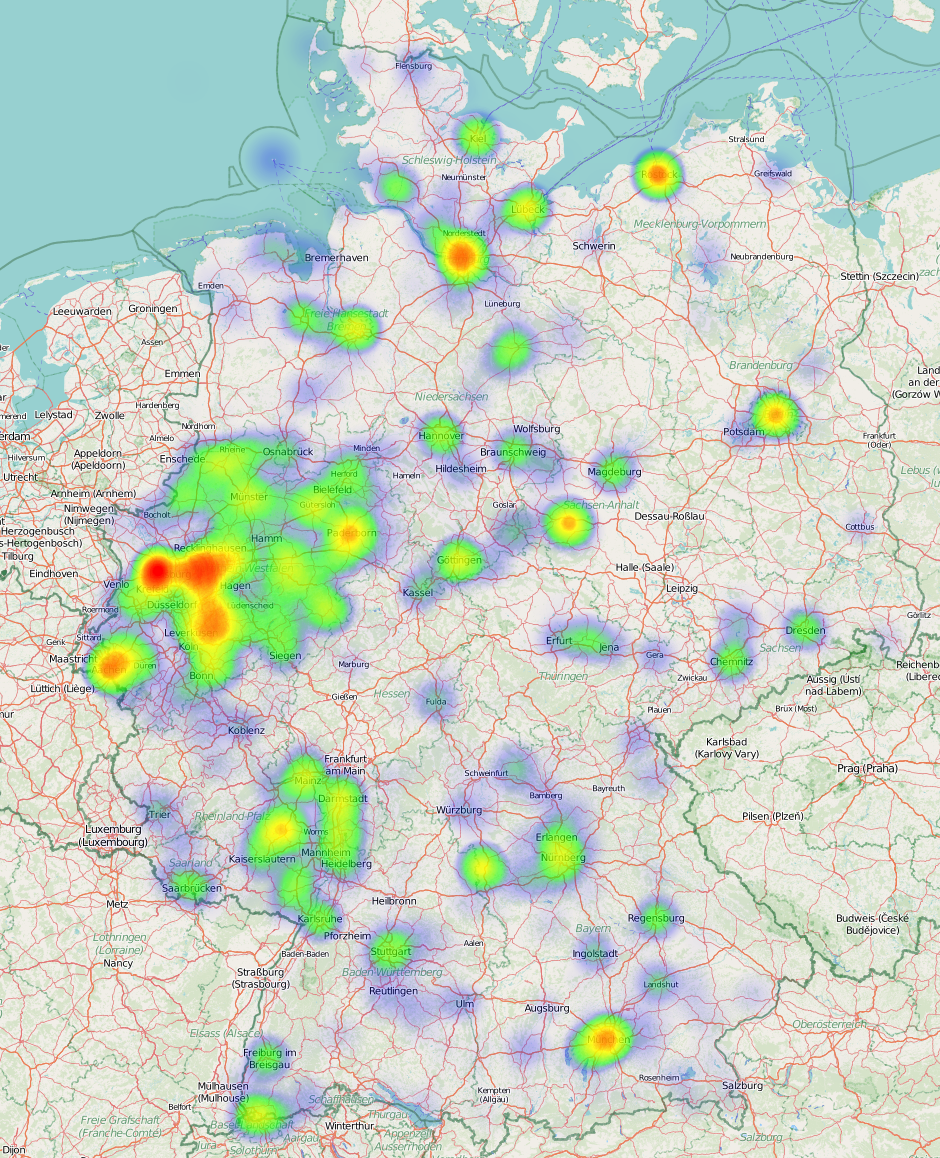
\includegraphics[width=\textwidth]{images/heatmap_germany.png} 
		\end{column}
	\end{columns}		
	\footnotetext[1]{Stand: 12.03.2016}

\end{frame}

\begin{frame}
\frametitle{Status Franken}
	\begin{itemize}
		\item ca. 50-300 aktive Freifunker: per eMail erreichbar und in der Mailingliste/Wiki aktiv
		\item etwa 2000 online Knoten
			\begingroup 
				\tiny{Stand 11.06.2017}
			\endgroup
		\item Ständig 3-4k Clients  
			\begingroup 
				\tiny{Stand 11.06.2017 - \href{https://monitoring.freifunk-franken.de/statistics}{Live Daten (Monitoring)}}
			\endgroup
	\end{itemize}
	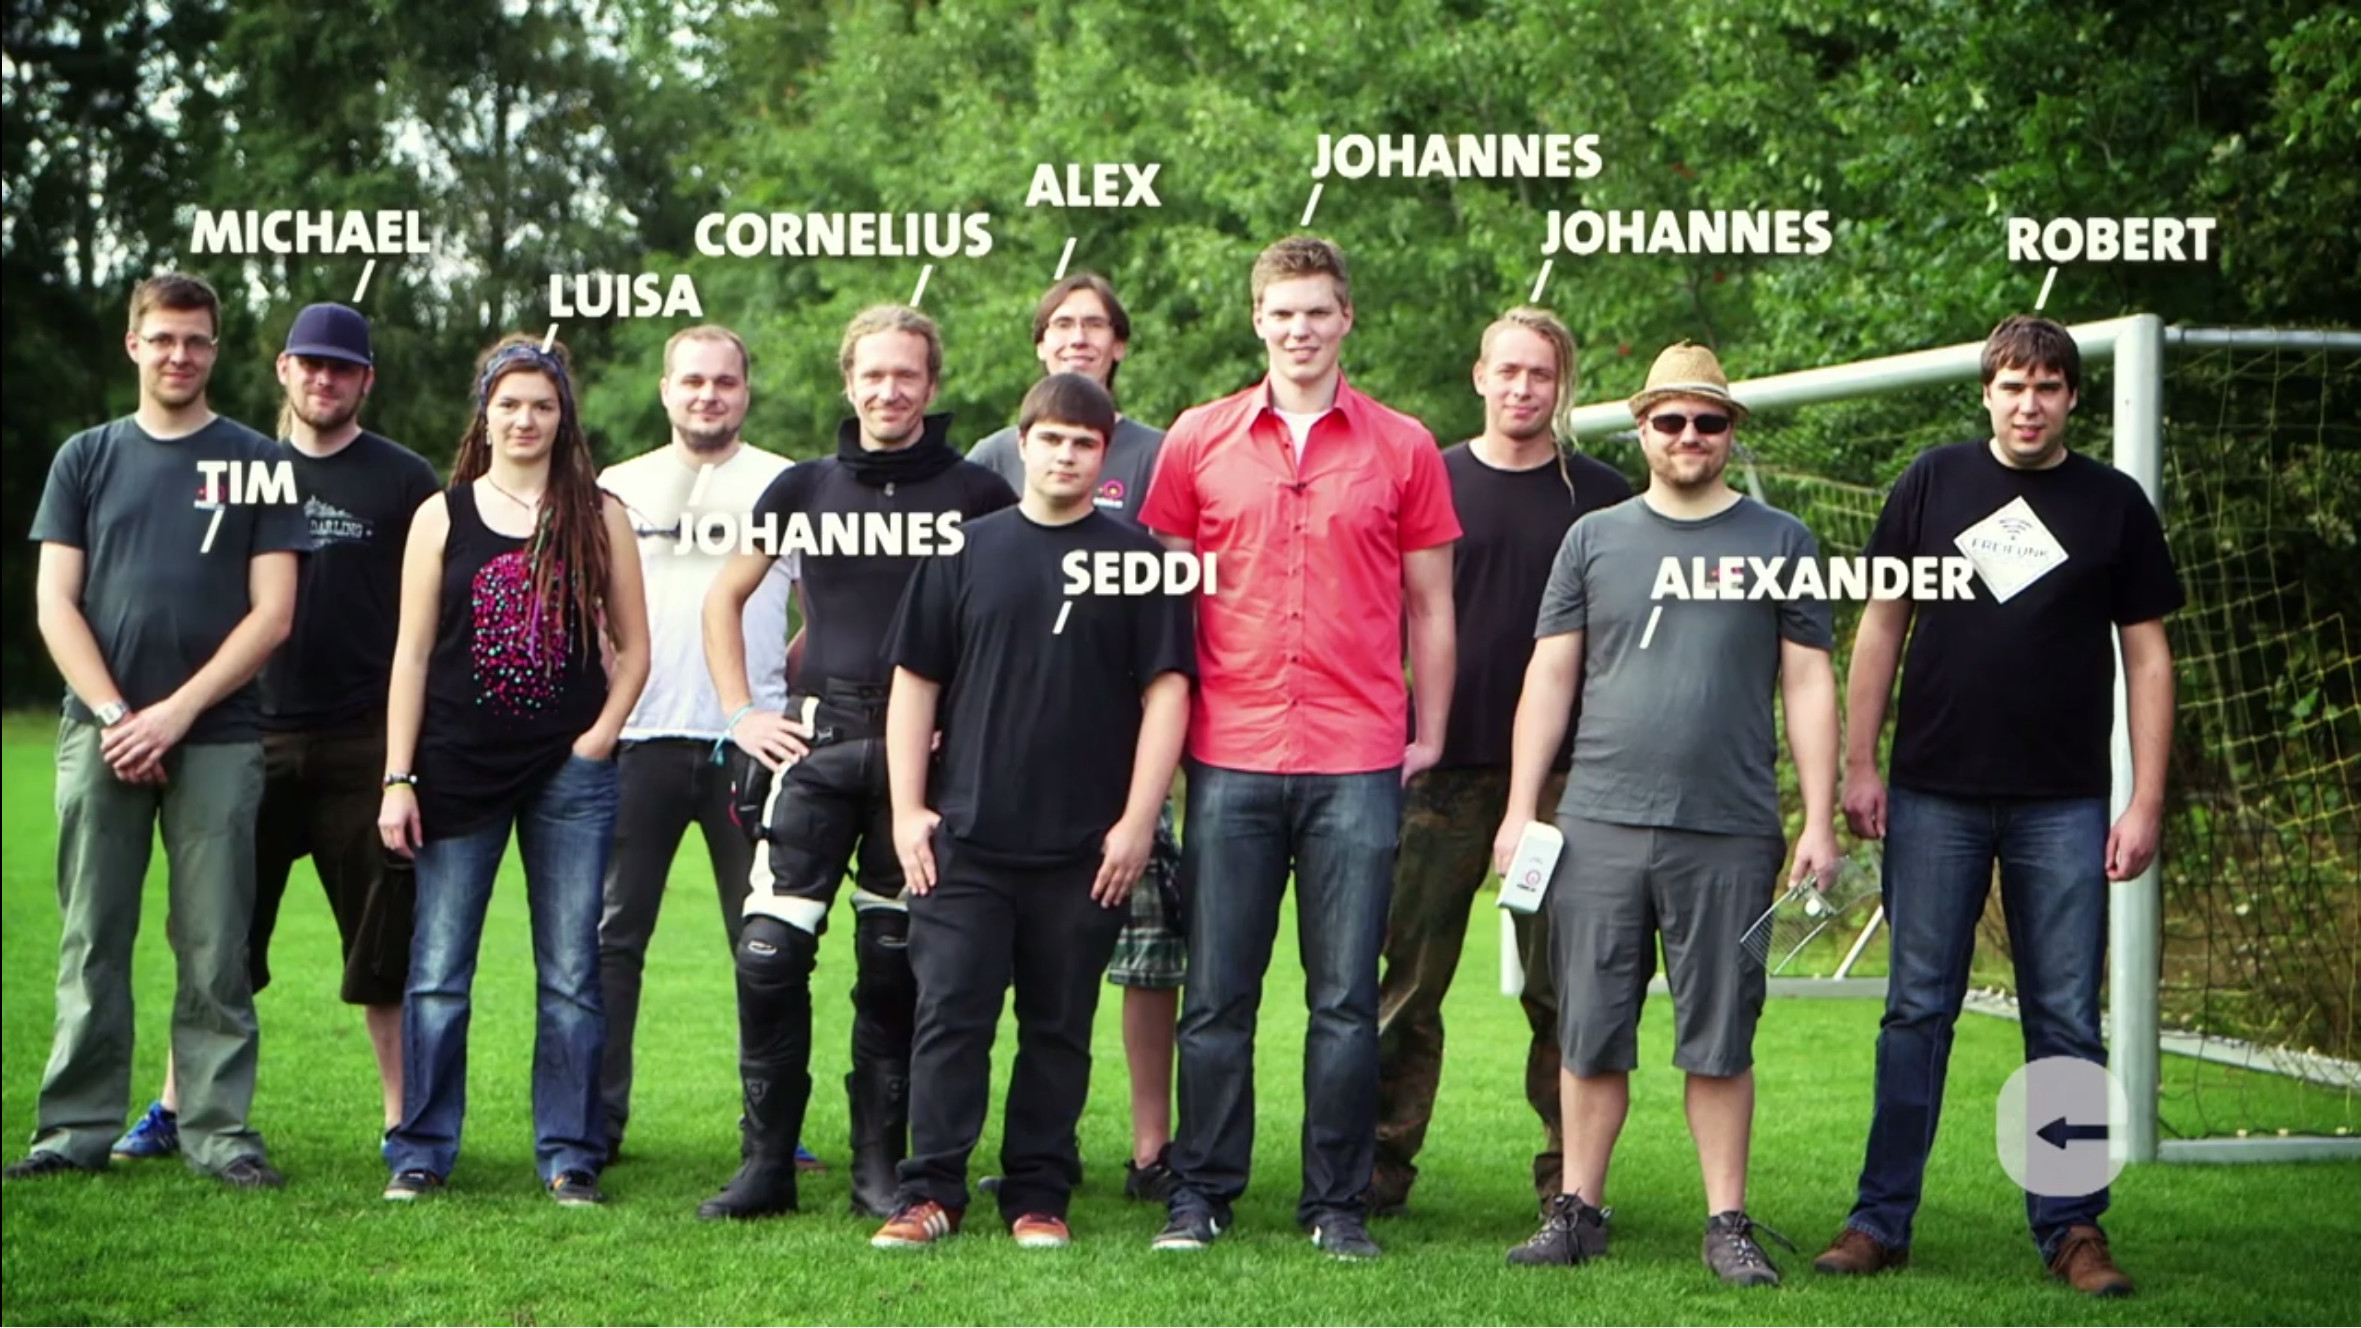
\includegraphics[width=\textwidth]{images/community.jpg}
\end{frame}

\subsection{Mitmachen!}

\begin{frame}
\frametitle{Mitmachen!}
	\begin{itemize}
		\item Anleitung gibt es im eigenen Wiki 
			\\ \href{https://wiki.freifunk-franken.de/w/Mitmachen}{https://wiki.freifunk-franken.de/w/Mitmachen}
		\item Mailingliste 
			\\ \href{https://wiki.freifunk-franken.de/w/Kommunikation}{https://wiki.freifunk-franken.de/w/Kommunikation}
		\item Netzverwaltung mit Karte: 
			\\ \href{https://monitoring.freifunk-franken.de}{https://monitoring.freifunk-franken.de}
	\end{itemize}
	\begin{flushright}
		
\includegraphics[scale=0.7]{images/CC-BY-SA.png}
		\begingroup \tiny{		
			\\CC-BY-SA März 2016 by delphiN, Casandro
			\\CC-BY-SA Mai 2016/Juni 2017 by b3yond}
		\endgroup
	\end{flushright}
\end{frame}